%!TeX spellcheck = en-US
\documentclass[../main.tex]{subfiles}
\begin{document}
\chapter{Analysis}
\label{chap:experimsetup}

Accessing real avionics hardware and software was out of my reach for this
research, therefore the analysis was carried out on open source implementations
of \textbf{ADS-B}, \textbf{FIS-B} and \textbf{NexRad} as found in some popular
source tree, binary package and device firmware releases such as Stratux,
FlightRadar24 and FlightAware. Experimenting on those software has also
secondary relevant implications as it allows to test at the same time avionics
protocols as well as IoT devices. As a matter of fact, even though avionics
software must comply with strict regulations and security standards as described
in DO-178 (ED-12 in Europe) and DO-278 (ED-109), it is most likely that using
one of the previously mentioned protocols as attack vector will have the same
effect on all implementations. While it is true that those systems are a crucial
component of an aircraft, as they are connected to the main control systems and
can take autonomous decisions, in the same way similar problems arise in ground
stations and in the network of IoT sensors as those can be used as an entry
point to an organization network.

Stratux project is particularly interesting as it uses inexpensive hardware (a
RaspberryPi and a RTL-SDR dongle) to provide \textbf{ADS-B In} services.
Moreover Stratux software is compatible with every major \acrlong{efb}s
(\acrshort{efb}) and, as far as it can be understood from its community, it is
largely used by pilots making it a proper avionics component at least in the
General Aviation sector.

Fuzzing was chosen as test method since, based on the knowledge acquired before
the research, no previous attempt of applying this test method to avionics
protocols had been carried out. This research gains even more importance if we
examine the latest news about the hacking of a Boeing 757 and the Cyber Grand
Challenge (CGC) 2016~\cite{CGC}. In particular, the CGC contained a specific
challenge (\texttt{FSK\_Messaging\_Service})~\cite{CGC-FSK} tailored to identify
techniques and systems able to discover vulnerabilities in the Radio Frequency
(RF) software using processed data after the RF front-ends. Aircraft and avionic
radio-communication interfaces are a perfect example of this type of design.
\textit{afl-unicron} has been proved particularly effective on solving this
specific challenge of the CGC, therfore it was used as an additional test
method.

Even though there is no official linking between the CGC and the Boeing hack the
circumstances indicate that there is a search and a need for knowledge and tools
that can exploit (and therefore eventually protect) RF facing software, embedded
devices in general and avionics and NextGen devices in particular. Researches in
this field are moving fast and some tools, such as beSTORM~\cite{bestorm} and
TumbleRF~\cite{tumblerf} that are now public, allow for direct RF fuzzing.

\section{Hardware Setup}

The hardware used during the research was the following:
\begin{itemize}

\item \textit{DVB-T (RTL-SDR) dongle:} a simple and cheap TV receiver equipped with the \emph{RTL2832U} or compatible chip can be tuned on a very wide range of frequencies, not only on the TVs.

\item \textit{RaspberryPi (RPi) 3 Model B:} was used to acquire the data using RTL-SDR dongles, and also to run some tests on the precompiled binaries. The RPi was running the latest version of Raspbian, or the particular flavor/version of Linux or Raspbian bundled as part of Stratux and FlightRadar24 SD-card firmware image files.

\item \textit{Standard laptop:} was used for dry-run testing, for initial code testing and for initial fuzzing experiments monitoring. The laptop has the following specifications: Intel Core i7 5500 (4 cores), 12 GB of RAM. Since the fuzzing is time and resource consuming, when the running experiments were considered promising or really important, they were moved to run on a multi-core server.

\item \textit{Multi-core server:} with the following specifications: Intel Xeon CPU E7-8837 @ 2.67GHz (64 cores, 32 cores used for a single afl-fuzz experiment), 1 TB of RAM, running Centos7.4 Linux.
\end{itemize}

\section{Software Setup}

The focus was on two of the most widespread and common implementations of the protocols: \emph{dump1090} and \emph{dump978}. The first one decodes \textbf{OldGen} and \textbf{1090ES} messages while the second one decodes \textbf{UAT} messages.

Those softwares have two main components:
\begin{enumerate}
  \item A \emph{demodulator} that converts the raw signal into a proper binary string.
  \item A \emph{decoder} that extracts the information from a packet provided by the demodulator.
\end{enumerate}

\emph{dump1090} handles directly the communication with the RTL-SDR dongle using
\emph{librtlsdr}. This library has been developed to work with the
\emph{RTL2832U} Radio Frequency (RF) chip providing access to the raw signal. It
is possible to define other sources for the raw data such as a file or the
standard input with the option \texttt{"-{}-ifile"}. \emph{dump1090} is a big
monolithic software which has undergone major rework and edits from different
authors resulting in many different forks. For these reasons testing each
component individually is a trivial task which can be accomplished only by using
\textit{afl-unicorn}.

\emph{dump978} does not acquire directly the raw data which, instead, has to be
provided on the standard input. \textit{librtlsdr} comes with a convenient
command line utility, called \textit{rtl-sdr}, which can be used to tune the
dongle on a specific frequency and dump the raw signal. The \textit{dump978}
software has a very modular design; in its basic version it is composed by at
least 3 different programs: \textit{rtl-sdr} used to communicate with the dongle
and acquire the raw data. \textit{dump978} which is the demodulator and takes
raw data as input giving encoded messages as output. \textit{uat2text} which is
the decoder and converts the output of the demodulator into a readable form. In
addition to these \textit{extract\_nexrad} extracts \textbf{NexRad} packets from
the demodulated output and \textit{plot\_nexrad.py} creates png images from
those data.

While \textit{dump978} is a compact and organized software with almost no forks
\textit{dump1090} has many different versions so testing all of them is
impossible. Therefore, three of the most widespread versions were selected for
fuzzing. The authors are \textit{Simone Sanfilippo (Antirez), MalcommRobb} and
the \textit{Stratux community}, for each author the very first and the latest
release were considered. The main \textbf{AFL} experiments were run on the
latest version of the tool from the Stratux repository as it seemed the most
updated and in active development. Later \textbf{AFL} tests were also carried
out on the first stable release from \textit{Antirez} (commit id 8236319) since
he is the original author of this tool and this commit keeps the basic features
without the clogging created by the later introduction of accessory tools such
as a server for real time view of the traffic. Moreover the testing wanted to
consider also precompiled binaries which are shipped inside the previously
mentioned Linux images and that are integrated in specific receivers such as the
proprietary ones from FlightRadar24. Therefore \textit{dump1090} was extracted
from the latest available release (1.4r4) and from the first working release
(0.8r2) of Stratux, as well as from the latest release (1.0.18-9) of the
FlightRadar24 Linux image (which is a free but not open source). The precompiled
version of \textit{dump1090} analyzed with \textit{afl-unicorn} was the one
contained in the first Stratux image and it seems to come directly from the
\textit{Antirez} repository and to be from the 8236319 commit.

All the collected sources were then compiled using \textit{afl-gcc} and
conveniently named using the following rule:
\emph{binary\_name--short\_commit\_id--repository\_name--version--vulnerability}
where the presence of the last value indicates that the binary contains an
artificially introduced vulnerability for testing purposes. The final lineup of
the binaries for testing can be seen in Figure \ref{fig:binline}.

 \begin{figure}[htp]
   \centering
   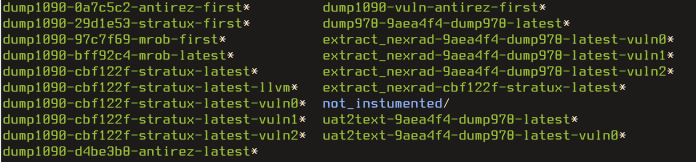
\includegraphics[scale=0.83]{images/binsetup.png}
   \caption{Binaries to be tested}
   \label{fig:binline}
 \end{figure}

\subsection{Datasets}

Every considered software requires its specific format of data, moreover, the
input given to \textbf{AFL} must be carefully chosen as using a too narrow input
(i.e. that triggers only a specific function) can lead to a waste of time before
the fuzzers actually is able to syntetize a meaningful input. Some suggestions
from the README of \textbf{AFL} and the ThalesIgnite
afl-training\footnote{\url{https://github.com/ThalesIgnite/afl-training}} are:

- Find some real inputs that exercise as much of the target as possible.

- Keep the input file small (Under 1kb  is ideal).

- Use multiple test cases only if they are functionally different from each
other.

\bigskip Complying with those rules, multiple test cases were created. A sample
for \textit{dump1090} was captured using the RaspberryPi placed in the
university laboratory and resulted in two files:  \emph{1090\_small.bin} which
contains a valid message, some noise and some invalid messages and
\emph{1090\_smaller.bin} which only contains one valid message. In addition to
this, \emph{modes1.bin} is a sample file contained in the \emph{dump1090}
repository. Despite containing some sample messages, however, it was never used
during the research. Capturing some 978MHz data is a hard task in Europe since,
as already said, this frequency and the \textbf{UAT} protocol is deployed mainly
in North America and China. Moreover no raw samples come with the
\textit{dump978} bundle but only some demodulated messages are provided. It was
therefore necessary to find another way of acquiring such data. One option was
to ask on Reddit which successfully resulted in more than half a GB
(\textit{978\_big.bin}) of raw capture containing almost any kind of
\textbf{UAT}
messages\footnote{\url{https://www.reddit.com/r/stratux/comments/7zdoaa/raw_dump_of_978_data}}.
Such a big file cannot be used as an input for \textbf{AFL} either because the
fuzzer will complain about the size and because using a such large amount of
data will have a significant impact on the fuzzing process and on the execution
speed of the binary. Therefore a smaller and more convenient file
(\textit{978\_random.bin}) was created, starting from the previous one and
taking some random data with the objective of simply reducing the size but still
keep at least one message. Creating files such as \textit{1090\_small.bin} and
\textit{978\_random.bin} was a trivial process since there is no easy way to
access and manage the raw data contained in the bigger files particularly
regarding the content and his meaning, however the creation of a tool to
interact and manages raw samples is left as future work.

To test \textit{uat2text} and \textit{extract\_nexrad} tools, some files were
created containing specific demodulated messages from \textit{978\_big.bin}. In
addition to this, two files (\textit{gdl90data} and \textit{gdl90data1})
containing \textbf{FIS-B/NexRad} samples from the documentation of the Garmin
first certified \textbf{ADS-B} datalink transceiver (GDL90~\cite{gdl90}) were
used in the tests. In particular for \textbf{FIS-B} services \acrshort{rtca}
provides a document (DO-358: \emph{``Minimum Operational Performance Standards
(MOPS) for Flight Information Services Broadcast (FIS-B) with Universal Access
Transceiver (UAT)''}) and the respective supplement containing many different
test files~\cite{do358} that, after a few modifications, can be used with
\textbf{AFL}.

The final content of the dataset directory can be seen in Figure \ref{fig:dataset}.

\begin{figure}[htp]
  \centering
  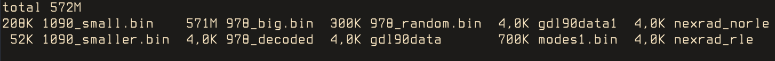
\includegraphics[scale=0.74]{images/dataset.png}
  \caption{Dataset created}
  \label{fig:dataset}
\end{figure}

\subsection{Tools}
\label{sec:tools}

As already mentioned \textbf{AFL} and \textit{afl-unicorn} were used for testing. However, during the project a dedicated set of tools and scripts were developed to partially automate and simplify data processing and fuzzing tasks.
The tools are divided into two categories: \textbf{Data Tools} used to manage, modify and create the datasets and \textbf{Fuzzing Tools} used to facilitate and speed up the fuzzing process. The details and descriptions of the tools are as follows:
\bigskip

\textbf{Data Tools}

\begin{itemize}

  \item \textbf{converter.sh} and \textbf{runner.sh} are scripts meant to
  interact with the data provided by the DO-358 supplement zip file. This
  archive contains many different files which are designed to be used with a
  dedicated test tool for real avionics hardware and software, for this reason
  there are 18 subfolders (called groups) and,  each one of them, contains:
  \textit{TestGroupXX Procedures.doc}, \textit{TestGroupXX Stimulus.csv} and a
  \textit{bin} folder with the actual data files. Every \textit{bin} folder has
  many different files, each representing a unique type of information which has
  already been demodulated and is stored in a binary format. Since the program
  being tested only accepts data in a uplink (or downlink) format
  \textbf{converter.sh} was written to convert one single file or an entire
  directory in the appropriate format. Every resulting file contains just one
  encoded type of data and, feeding a large amount of those files into a
  program will be a long and tedious task. For this reason the
  \textbf{runner.sh} script will feed each file contained inside a specified
  directory through the user defined program either interactively, namely
  stopping after each file and asking if the user wants to continue, or simply
  running all files at once.

  \item \textbf{message\_generator.py} is a simple script that after receiving
  the first part of a demodulated Mode-S message can calculate a correct CRC.
  This can be done virtually for every random string with a correct length but
  the script has not been widely used.

  Its only application was for test purposes since it was considered interesting
  to see what could happen when the program being tested was fed with particular
  messages such as those composed by all 1 or all 0 and having a valid CRC. This
  script could be part of a future bigger program that will test the protocols
  generating messages that always have a valid CRC.

\end{itemize}

\bigskip
\textbf{Fuzzing Tools:}

\begin{itemize}

  \item \textbf{start.sh} is a script that will automatically spawn or resume a
  user defined number of fuzzers. In particular since \textbf{AFL} can be
  parallelized on many cores the script handles the creation of the input and
  output folders as well as a convenient naming of each fuzzer instance. It will
  take as input the number of cores to be used and all the other parameters
  required by the fuzzer, perform a check of the directories and then start the
  chosen number of fuzzers: 1 Master and $n-1$ Slaves.

  \item \textbf{unicorn\_template\_generator.py} will create the template for
  the Unicorn Engine and populate it with all the required addresses such as the
  ones inside which the emulation should take place or the one of the functions
  to be skipped. The script is designed to be sourced inside a running session
  of GDB while the program is on a breakpoint inside a function; it will not
  work if called inside the main since it is specifically designed to search for
  the end of the function.

  \item \textbf{extract\_from\_memory.py} will dump the specified memory region
  from a running program in GDB to be used as input for \texttt{afl-unicorn}.
  This will generate a file that can be used with the previously generated
  template, this will perform the various mutations and then  load it in the
  proper memory region.

  \item \textbf{afl utility scripts}:

  \begin{itemize}

    \item \textbf{killem\_afl.sh} $\rightarrow$ stop a running instance of afl.

    \item \textbf{wazzup\_afl.sh} $\rightarrow$  get information and statistics on the running instances of the specified fuzzer.

    \item \textbf{afl\_noroot.sh} $\rightarrow$ run afl on a system where the user does not have root privileges.

  \end{itemize}

\end{itemize}


\section{Proceedings}

The analysis was first done on the \textbf{OldGen/1090ES} then on \textbf{UAT}.
As already said the first step was to confirm that the fuzzer was working
correctly and that it was able to crash the analyzed binaries. For this task
some synthetic vulnerabilities were introduced in almost all the binaries
starting from \textit{dump1090}. The vulnerability had to be kept simple,
powerful and yet easy to trigger, for this reason a simple buffer overflow was
chosen. It is important to note that the synthetic vulnerability should not be
triggered by the initial test case provided to \textbf{AFL} otherwise it will
stop the fuzzing considering the binary not reliable.

The integration in only one binary of all the functions of \textit{dump1090} had
an impact on the performances of the fuzzer and made correctly test the
demodulator and the decoder parts harder as the data had always to be
demodulated first. This lead to some inconveniences: first of all it was harder
to feed arbitrary data directly to the decoder as no modulator was available.
Then, even just to test the decoder, raw data had to be supplied resulting in a
useless demodulation step and in a waste of time as many mutations will have no
effect and will be processed as random noise. Although it is possible to feed
encoded messages to \textit{dump1090} this is done thought a socket connection
which requires a network fuzzer and is out of the scope of this research.

Three vulnerabilities were introduced in different parts of the latest
\textit{dump1090} release from the Stratux repository as it can be seen in
Figure \ref{fig:1090vuln}. The overflow was inside the decodeModesMessage
function, the second one was inside the decodeExtendedSquitter function while
the last one was in the printing function, the demodulator was not touched as,
without specific knowledge, it is not easy to understand which part would be the
best.

\begin{figure}[htp]
\centering
\begin{minipage}{.5\textwidth}
  \centering
  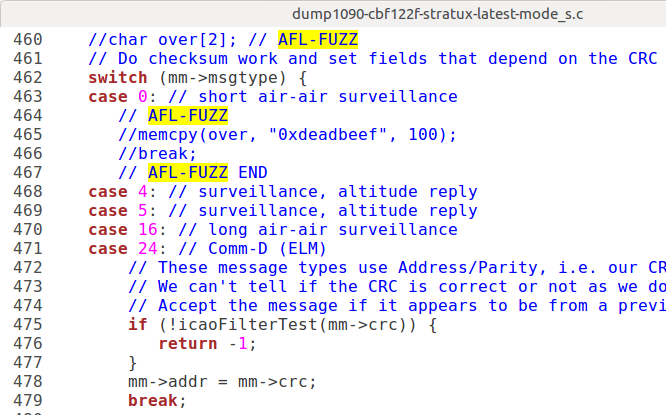
\includegraphics[scale=0.4]{images/src_dump1090-cbf122f-stratux-latest-vuln0.png}
\end{minipage}%
\begin{minipage}{.5\textwidth}
  \centering
  \vspace*{-0.22in}
  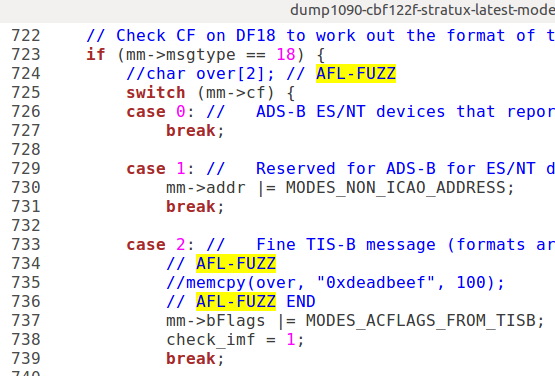
\includegraphics[scale=0.4]{images/src_dump1090-cbf122f-stratux-latest-vuln1.png}
  \end{minipage}\\
  \begin{minipage}{.5\textwidth}
    \hspace*{-0.3in}
    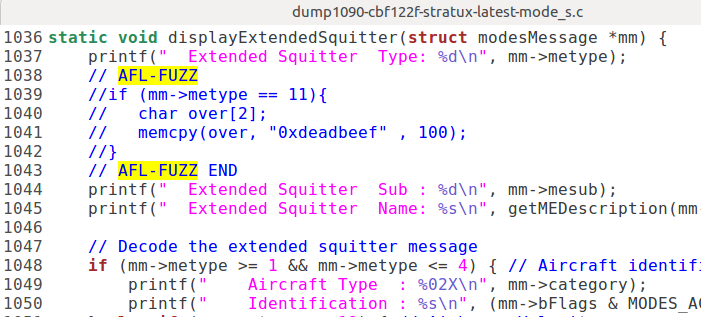
\includegraphics[scale=0.45]{images/src_dump1090-cbf122f-stratux-latest-vuln2.png}
    \end{minipage}\\
\caption{dump1090 vulnerabilities}
\label{fig:1090vuln}
\end{figure}

\textit{1090\_small.bin} was then used to test the vulnerable binaries using 32
instances of \textbf{AFL} (1 Master 31 Slaves) for each of the 3 binaries, one
per vulnerability. Interestingly the fuzzer was able to crash only the first
binary, there could be multiple reasons for this as it will be discussed in
Chapter \ref{chap:resconc}.

Since even after a large amount of cumulative execution days the fuzzer was not
able to find any vulnerability in the latest version of \textit{dump1090} from
the Stratux repository (short commit id \textit{cbf122f}) using
\textit{1090\_small.bin} even with non instrumented binaries and the QEMU mode
of \textbf{AFL} the focus was shifted on another approach: \textit{afl-unicorn}.
Therefore it was necessary to understand how templates for this tool are
generated, luckily a basic blank template comes inside the \textit{afl-unicorn}
repository along with a tool to dump the memory content and addresses. Using GDB
with the GEF\footnote{GDB Enhanced Features - https://github.com/hugsy/gef}
plugin the template was in the beginning created by had and set to test the
\textit{detectModeS} function (in Figure \ref{fig:detectms}) which is
responsible of demodulating Mode S messages. Getting to a basic working version
of the template is not an easy task since many of the libraries used by
\textit{dump1090} relays on System Calls which, since no underlying operating
system is present inside the emulator, will cause unpredictable crashes.
Therefore it was necessary to find the addresses of problematic functions, such
as \textit{printf, putchar, puts} and so on, and to configure hooks in order to
skip such functions.

\begin{figure}[htp]
  \centering
  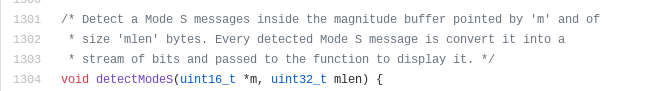
\includegraphics[scale=0.9]{images/detectModeS.png}
  \caption{detectModeS function}
  \label{fig:detectms}
\end{figure}

This analysis was carried out on the ARM precompiled binary contained in the
first release of the Stratux Linux image (stratux-v.0.1-08072015). For future
templates the above mentioned \textit{unicorn\_template\_generator.py} was used.
To confirm that \textit{afl-unicorn} was working as expected a vulnerable
version of \textit{dump1090}, having an overflow inside the \textit{detectModeS}
function, was compiled on the RaspberryPi and the context dumped with the
mentioned script. Then the fuzzer was run on the resulting template an entire
day on the standard laptop, unluckily no crashes where produced both for the
vulnerable and for the stock versions. This might be due to the low hardware
resources of the regular laptop and to the low testing time since
\textit{afl-unicorn} has a much slower testing speed due to the many steps
required by the Unicorn Engine to start the emulation and to the low emulation
speed. For unknown reasons it was not possible to have a working instance of the
Unicorn Engine and therefore of \textit{afl-unicorn} on the multicore server
since the execution of the emulation engine on an x86 and an x86\_64 machine
gives completely different results than the runs on the server.

Moving on from \textit{dump1090} the research focused on \textit{dump978}, an
experimental run of \textbf{AFL} was done using \textit{978\_random.bin} and the
latest version of \textit{dump978} (short commit id \textit{9aea4f4}). However,
the 978 demodulator was not the main target of the research but it was more
focused on \textit{uat2text} and \textit{extract\_nexrad}, this last software is
of particular interest as it is designed to handle packets containing images
which can be encoded, among others, also with Huffman algorithm known through
the years to be particularly difficult to implement in a safe
way~\cite{cve20176890, cve20074537}. To test those software the same approach as
before was used, meaning that \textbf{AFL} was at first run on an artificially
vulnerable version and then on the stock release. This resulted in three
binaries, two from \textit{extract\_nexrad} and one from \textit{uat2text}, each
containing a vulnerability in a different part of the code, as it can be seen in
Figure \ref{fig:978vuln}.

\begin{figure}[htp]
\centering
\begin{minipage}{.5\textwidth}
  \centering
  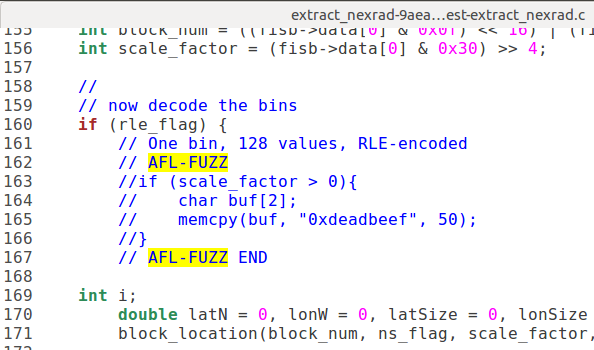
\includegraphics[scale=0.4]{images/src_extract_nexrad-9aea4f4-dump978-latest-vuln0.png}
\end{minipage}%
\begin{minipage}{.5\textwidth}
  \centering
  \vspace*{-0.033in}
  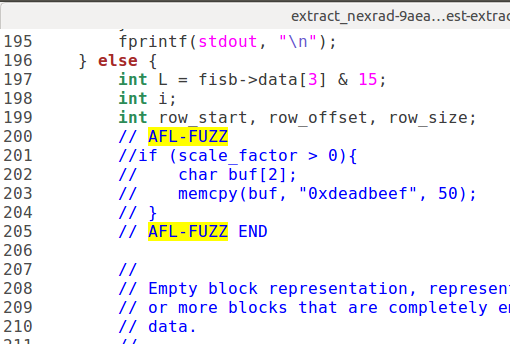
\includegraphics[scale=0.4]{images/src_extract_nexrad-9aea4f4-dump978-latest-vuln1.png}
  \end{minipage}\\
  \begin{minipage}{.5\textwidth}
    \hspace*{-0.3in}
    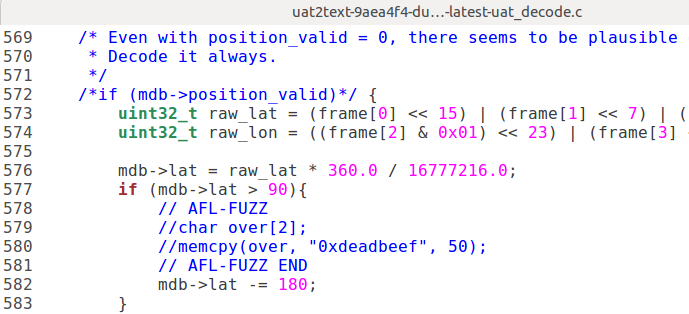
\includegraphics[scale=0.45]{images/src_uat2text-9aea4f4-dump978-latest-vuln0.png}
    \end{minipage}
\caption{extract\_nexrad and uat2text vulnerabilities}
\label{fig:978vuln}
\end{figure}

The first vulnerability in \textit{extract\_nexrad} is inserted to cause an
overflow if the data is RLE encoded and the scale factor is greater than 0, this
value can go from 0 to 2. The second vulnerability is triggered if the data is
not RLE encoded and the scale factor is greater than 0. Although it is
theoretically possible to send Huffman Encoded \textbf{NexRad} images no
reference to Huffman Tables or Huffman Decoding was spotted in the source code.

In \textit{uat2text} the vulnerability was put in the
\textit{uat\_decode\_uplink\_mdb} function, this is where the decoding of
\textbf{UAT} frames takes place, the vulnerability is triggered if the decode
latitude is greater than 90 degrees.

The fuzzer was successfully run on both vulnerable versions of
\textit{extract\_nexrad} using \textit{nexrad\_rle} and \textit{nexrad\_norle}
files, \textbf{AFL} was able to crash the two versions in a very short amount of
time. After this the fuzzer was run on the stock version using the same two
files however, even after many days of cumulative execution, no crash was
triggered.

\textit{uat2text} was then tested using \textit{978\_decoded} as input, even in
this case \textbf{AFL} was able to crash the vulnerable binary almost instantly.
However, when run on the stock binary using the same file as input, many days of
cumulative execution produced no appreciable crash.

A last test, using a completely different binary found in
\textit{afl-demo}\footnote{https://gitlab.com/wolframroesler/afl-demo}
repository, was carried out on all the flavours of \textbf{AFL} used during the
research. This binary is built specifically to test the abilities of the fuzzer
and is a simple and buggy URI decoder. It was run on just a single instance of
\textbf{AFL}, \textbf{AFL} QEMU mode and \textit{afl-unicorn}. The results can
be seen in Figure \ref{fig:afldemo}.

\begin{figure}[htp]
\centering
\begin{minipage}{.5\textwidth}
  \centering
  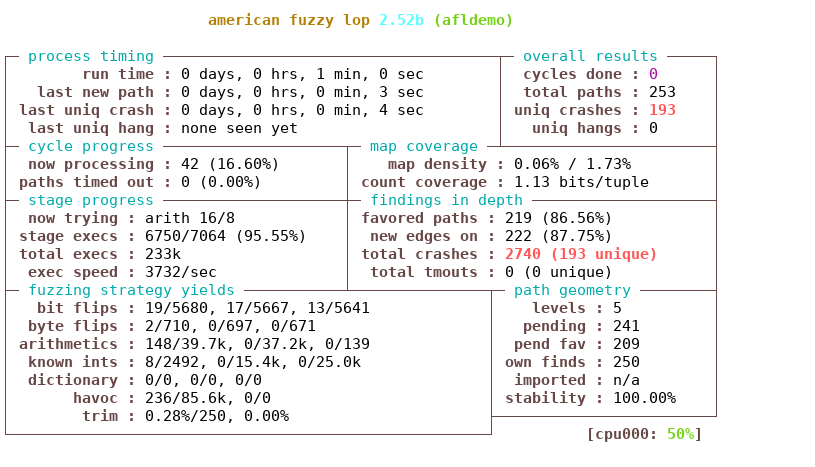
\includegraphics[scale=0.4]{images/afl-test_x86_64-white.png}
\end{minipage}%
\begin{minipage}{.5\textwidth}
  \centering
  \vspace*{-0.033in}
  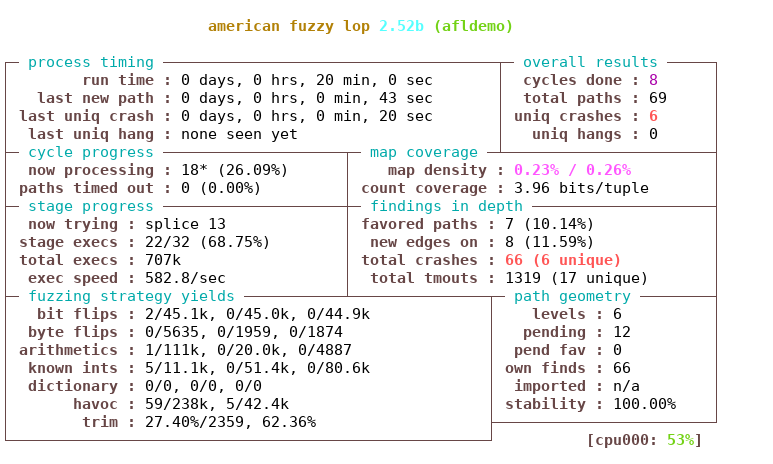
\includegraphics[scale=0.4]{images/afl-test_qemu.png}
\end{minipage}\\
\begin{minipage}{.5\textwidth}
  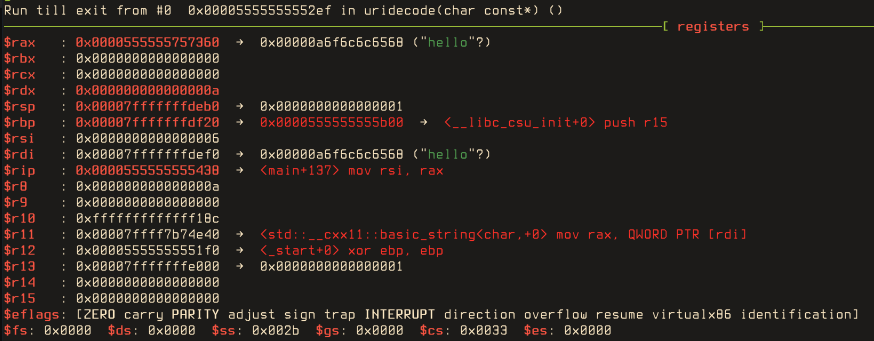
\includegraphics[scale=0.48]{images/gdb_afl-test_unicorn.png}
\end{minipage}%
\begin{minipage}{.5\textwidth}
  \flushright
  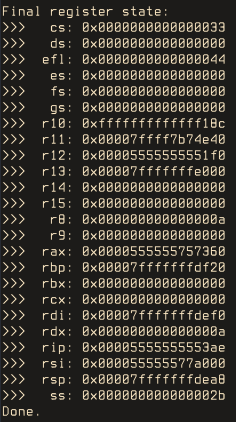
\includegraphics[scale=0.5]{images/unicorn_afl-test.png}
\end{minipage}\\
\begin{minipage}{.5\textwidth}
  \centering
  \hspace*{-0.3in}
  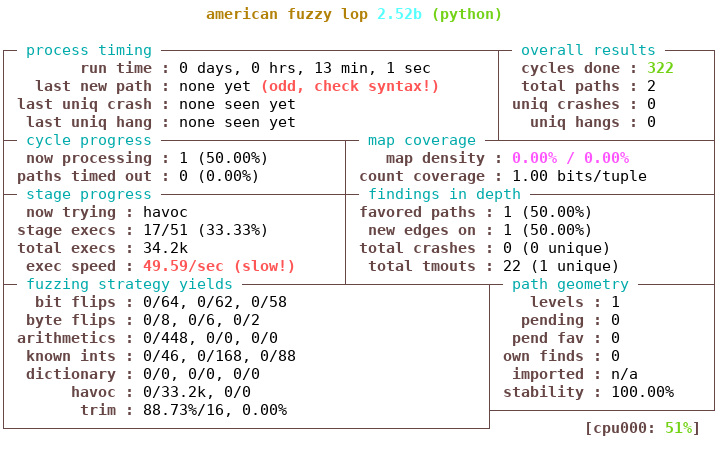
\includegraphics[scale=0.48]{images/aflunicorn_no_crash.png}
\end{minipage}
\caption{comparative test with afl-demo}
\label{fig:afldemo}
\end{figure}

The top left image shows the results after a 1 minute run of \textbf{AFL}, which
in such a short amount of time is able to discover 193 unique crashing inputs.
The top right image shows the results of a 20 minutes run of \textbf{AFL} on a
BlackBox binary using QEMU mode. As it can be clearly seen this approach is way
slower than the previous one as a matter of fact it was able to find only 6
unique crashes. The last three images are about \textit{afl-unicorn}, as it can
be seen from the last one it is not able to find any crashes and, most
importantly, no new paths are triggered. This might be due to many different
factors that still need further and deeper investigation. Although the two
previous images show that the real registers, after the exectuion of the tested
function (\textit{uridecode}), from inside GDB and the ones resulting from the
execution of Unicorn template have the same value except for some of them that
are related to the address of where the input is loaded.

\end{document}
